\documentclass{article}

\usepackage[preprint]{neurips_2023}

\usepackage[utf8]{inputenc} % allow utf-8 input
\usepackage[T1]{fontenc}    % use 8-bit T1 fonts

\usepackage{microtype}      % microtypography

% \usepackage{url}            % simple URL typesetting
\usepackage{xurl}
% \usepackage{hyperref}       % hyperlinks
\usepackage[colorlinks=true, linkcolor=blue, urlcolor=cyan]{hyperref}

\usepackage{enumitem}

\usepackage{booktabs}       % professional-quality tables

\usepackage{graphicx}
\usepackage{subcaption}
\usepackage{float}

\title{Internship Research Project Report}

\author{%
  Yu Du \texttt{(Student ID: 24213100)} \\
  \texttt{yu.du2@ucdconnect.ie} \\
  \href{https://github.com/Godot008/UCD_MEIN40420_Internship_Research_Project_2024-25-Summer}{\texttt{github.com/Godot008/Internshi\_Project}}
}

\begin{document}

  \maketitle

  \begin{abstract}
    The PD-1 immune checkpoint pathway plays a pivotal role in regulating T cell activation and maintaining immune homeostasis. A deeper understanding of the dynamic proteomic changes following PD-1 engagement is essential for uncovering potential biomarkers and therapeutic targets, as well as elucidating mechanisms of immune checkpoint inhibitor (ICI) resistance. In this project, I performed quantitative proteomic profiling of PD-1 reporter and control conditions at three time points (5 minutes, 20 minutes, and 4 hours) after TCR stimulation. Raw abundance data were processed through coverage and abundance filtering, log2 transformation, and batch effect correction using ComBat. Differential expression analysis was followed by hierarchical clustering, pathway enrichment, and STRING protein-protein interaction (PPI) network visualization. In this project, I performed quantitative proteomic profiling of PD-1 reporter and control conditions at three time points (5 minutes, 20 minutes, and 4 hours) after TCR stimulation. Raw abundance data were processed through coverage and abundance filtering, log2 transformation, and batch effect correction using ComBat. Differential expression analysis was followed by hierarchical clustering, pathway enrichment, and STRING protein-protein interaction (PPI) network visualization. A total of 16 significantly regulated proteins were identified. Time-resolved clustering revealed distinct expression modules, with one cluster enriched in ribosomal and metabolic processes (e.g., RPL22, CS, PLG), while another cluster highlighted immune-related pathways and chromatin-associated proteins (e.g., HBA2, H2AC21). Enrichment analyses demonstrated associations with pathways such as ribosome function, viral defense, necroptosis, and complement cascades, with FDR correction enhancing the robustness of biologically meaningful modules. STRING PPI analysis further identified key hub proteins (e.g., RPL22, HBA2, H2AC21) that may serve as central regulators in PD-1-mediated immune modulation. These results provide proteomic-level evidence that PD-1 activation reshapes TCR signaling in a temporally dynamic manner. By identifying functionally enriched protein clusters and network hubs, this work advances our understanding of ICI mechanisms, offers new insights into resistance development, and highlights candidate proteins as potential therapeutic targets.
  \end{abstract}

  \section{Introduction}

    In recent years, cancer immunotherapy has made remarkable advances, aiming to enhance the immune system's ability to recognize and eliminate tumor cells, thereby improving the specificity and durability of anticancer responses (Han et al., 2020). Among immune checkpoints, programmed cell death protein 1 (PD-1) is a pivotal inhibitory receptor and a major target of immune checkpoint inhibitors (ICIs). Binding of PD-1 to its ligands (PD-L1 and PD-L2) suppresses T cell receptor (TCR)-mediated signaling and modulates multiple key pathways, ultimately impairing T cell activation. Tumor cells often exploit this mechanism to evade immune surveillance (Mizuno et al., 2019; Chen et al., 2025).

    While transcriptomic studies have revealed aspects of PD-1-related signaling, they primarily capture transcriptional regulation and cannot directly reflect functional effectors or post-transcriptional regulation. Proteomics, in contrast, directly measures the functional molecular landscape, providing quantitative information on protein abundance, post-translational modifications, and dynamic signaling processes. This makes proteomic profiling particularly valuable for elucidating PD-1 signaling mechanisms.

    In this internship research project, I utilized quantitative whole-proteome data\footnote{I have stored the original data, generated intermediate data and result data on my Google Drive at UCD (\url{https://drive.google.com/drive/folders/1-tbezxn0ImQxPkNMIwaoOBjEl7V8tOTd?usp=share_link}) for reference.} of the Jurkat T cell line\footnote{This cell line is widely used as an in vitro model for T cell signaling studies due to its high reproducibility.} acquired via mass spectrometry using the MaxLFQ algorithm, under PD-1 stimulation at multiple time points (5 min, 20 min, 4 h). I systematically investigated the temporal dynamics of protein expression, including: 
    \begin{enumerate}
      \item Differential protein identification with time-integrated analysis; 
      \item Clustering-based detection of early- and late-response patterns; 
      \item Gene Ontology (GO) and Kyoto Encyclopedia of Genes and Genomes (KEGG) enrichment analyses to reveal associated biological processes and pathways; 
      \item Construction of protein-protein interaction (PPI) networks to identify potential key regulators.
    \end{enumerate}

    This work aims to elucidate the effects of PD-1 activation on TCR signaling and downstream immune regulation, providing proteomic-level evidence to advance our understanding of ICI mechanisms, resistance development, and the discovery of novel therapeutic targets.

  \section{Methods}

    \subsection{Data Sources and Data Pre-Processing}

      The proteomic dataset used in this project was obtained from quantitative mass spectrometry (MaxLFQ method) of Jurkat T cells, including PD-1 reporter and control groups at three time points: 5 min, 20 min, and 4 h. 

      Pre-processing steps were as follows:

      \begin{enumerate}
        \item Data formatting to retain only relative abundance values and ensure compliance with first normal form (1NF).
        \item \textbf{Coverage filtering:} removing proteins with >50\% missing values.
        \item \textbf{Abundance filtering:} removing proteins with low total abundance across all samples, based on the initial dataset size (6,270 proteins) and observed abundance distribution.
        \item \textbf{Batch effect correction:} batch information was extracted from sample IDs (ProtA-ProtD) using regular expressions and recorded in the metadata table; applying \texttt{scanpy.pp.combat()} on log2-transformed data, using batch (A-D) as the primary variable and experimental condition and time point as covariates; PCA was performed before and after batch correction, and PC1-PC2 scatter plots were generated to evaluate the removal of batch effects while retaining biological separation.
        \item \textbf{Outlier handling:} applying winsorization (upper/lower bound trimming) or removing proteins with Z-scores > 5 for specific analyses;
        \item \textbf{Standardization:} prior to heatmap plotting, applying row-wise Z-score standardization (\texttt{standard\_scale=1}) and selecting the top 30 most significant proteins for visualization.
      \end{enumerate}

    \subsection{Differential Expression Analysis}
    
      To compare protein expression differences between the PD-1 reporter group and the control group at each time point, Welch's t-test was applied to calculate the statistical significance (p-values) for each protein, followed by false discovery rate (FDR) correction using the Benjamini-Hochberg method. Both unadjusted results (p < 0.05) and FDR-adjusted results (FDR < 0.1) were retained to allow for direct comparison of findings under different significance criteria in the Results section. The thresholds for log2 fold change (log2FC) were set as follows: absolute log2FC > 1.0 for unadjusted results and > 0.5 for FDR-adjusted results, where log2FC was defined as the log2-transformed difference between group mean abundances.

      Following the identification of differentially expressed proteins, they were further classified into upregulated and downregulated (negatively regulated) proteins based on the sign of log2FC, thereby clarifying the direction of expression change under each condition. To obtain a comprehensive set of differentially expressed proteins, results from the three time points were combined, and any protein significant at least at one time point was retained to capture time-specific changes and avoid omitting potentially important candidates.

    \subsection{Functional and Pathway Enrichment Analysis}

      {\sloppy
        For each protein cluster, pathway enrichment analysis was performed using the \texttt{gseapy.enrichr()} function against Reactome, Gene Ontology (GO), and Kyoto Encyclopedia of Genes and Genomes (KEGG) databases. This method employs Fisher's exact test to calculate enrichment significance.
      \par}

    \subsection{Protein-protein interaction (PPI) network}

      Gene sets of significant proteins were queried against the STRING database (v11.5) API for human proteins (taxon ID: 9606) with a minimum interaction confidence score of 0.4. If no interactions were found, the threshold was automatically lowered to 0.15, and first-shell neighbors could optionally be added to expand the network. Isolated nodes were retained in the visualization to ensure complete representation of the input proteins, facilitating comprehensive interpretation of network structure and potential regulatory relationships.

    \subsection{Clustering and Visualization}

      Hierarchical clustering was performed on standardized expression values of significant proteins. The optimal number of clusters was determined using dendrogram inspection combined with biological interpretation. Heatmap clustering was used to identify early- and late-response protein expression patterns.

  \section{Results}

    \subsection{Data Sources and Data Pre-Processing}

      After applying combined coverage and abundance filtering, the number of proteins was reduced from the initial 6,270 to 866 (Figure \ref{fig:abundance_distribution_comparison}). As shown in the abundance distribution histograms, the raw data exhibited a strong bias with most proteins concentrated in the low-abundance range, whereas after filtering, low-abundance noise was effectively removed and the overall distribution became more balanced, thereby improving the robustness of downstream analyses (Figure \ref{fig:abundance_distribution_before} vs. \ref{fig:abundance_distribution_after}).
      
      \begin{figure}[H]
        \centering
        \begin{subfigure}{0.45\textwidth}
            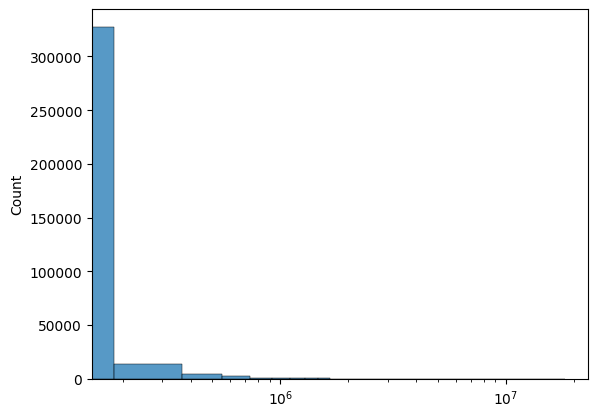
\includegraphics[width=\linewidth]{figures/abundance_distribution_before.png}
            \caption{Original abundance distribution.}
            \label{fig:abundance_distribution_before}
        \end{subfigure}
        \hfill
        \begin{subfigure}{0.45\textwidth}
            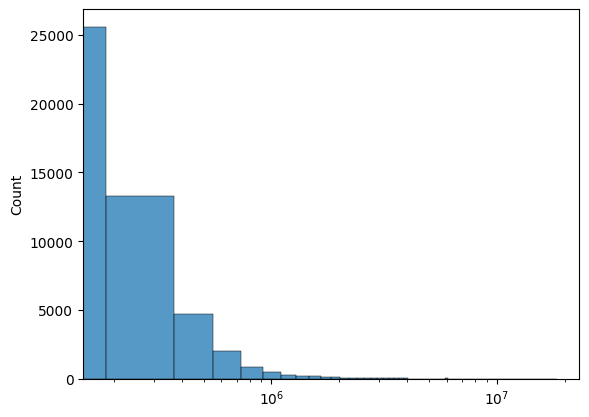
\includegraphics[width=\linewidth]{figures/abundance_distribution_after.png}
            \caption{Filtered abundance distribution.}
            \label{fig:abundance_distribution_after}
        \end{subfigure}
        \caption{Comparison of protein abundance distribution before and after filtering.}
        \label{fig:abundance_distribution_comparison}
      \end{figure}
      
      Subsequently, batch correction was performed using the ComBat method. Before correction, PCA revealed a clear separation of samples driven by batch effects, indicating that batch variation had a substantial influence on the data structure. After correction, the separation by batch was greatly reduced and samples from different batches were well mixed, while the biological separation trend remained preserved. This demonstrates that batch correction effectively removed non-biological variation (Figure \ref{fig:pca_combat}, left vs. right). 

      \begin{figure}[H]
        \centering
        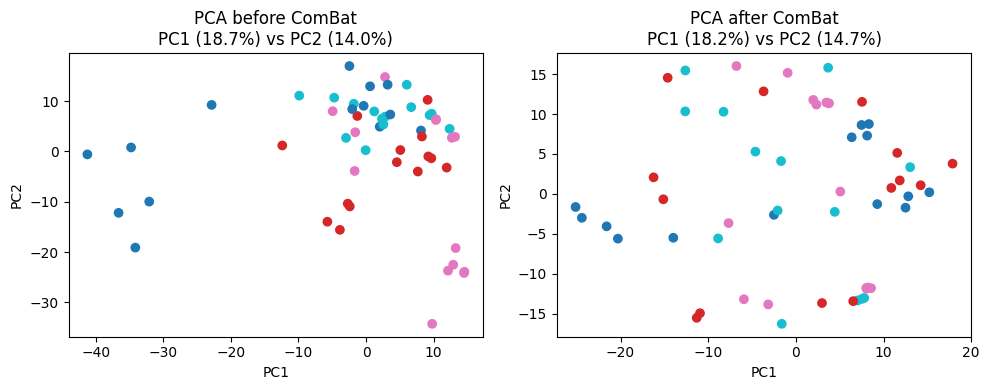
\includegraphics[width=0.8\textwidth]{figures/pca_combat.png}
        \caption{Comparison of PCA test results before and after batch correction.}
        \label{fig:pca_combat}
      \end{figure}

    \subsection{Differential Expression Analysis}

      In the differential expression analysis, I compared the PD-1 activated group with the control group at three time points: 5 minutes, 20 minutes, and 4 hours (Table \ref{tab:pd1_results}). At the raw p-value threshold, several proteins were found to be significantly different at 5 minutes, including HNRNPLL, CACTIN, HBD, and SORL1. After FDR adjustment, the number of significant proteins was reduced, but notable hits such as PLG, HBA2, EWSR1, and H2AC21 remained significant. At 20 minutes, BLTP3A and LNPK showed significance under raw p-values but did not pass FDR correction. In contrast, at 4 hours, a larger set of stable differentially expressed proteins was identified. For example, RPL22 was significant under both raw and adjusted criteria, while proteins such as CS, BTF3, EIF6, RPL18A, and NUDT5 emerged as significant only after FDR correction.

      \begin{table}[H]

        \centering

        \caption{PD-1 differential expression analysis results at multiple time points.}
        \label{tab:pd1_results}

        % ---- 5 minutes ----
        \subcaption*{5 minutes}
        \begin{tabular}{lrrrrr}
          \toprule
          Gene & log2FC & p\_value & p\_fdr & significant & significant\_fdr \\
          \midrule
          \multicolumn{6}{l}{\textit{Raw results}} \\
          HBD      &  1.2808 & 0.0276 & 0.3023 & True  & False \\
          H2BC20P  &  1.0544 & 0.0091 & 0.1727 & True  & False \\
          CACTIN   & -1.7535 & 0.0345 & 0.3166 & True  & False \\
          HNRNPLL  &  1.1090 & 0.0461 & 0.3380 & True  & False \\
          SORL1    &  8.5232 & 0.0159 & 0.2202 & True  & False \\
          \midrule
          \multicolumn{6}{l}{\textit{FDR-adjusted results}} \\
          PLG     & 0.7115 & 3.21e-07 & 0.000275 & False & True \\
          HBA2    & 0.7566 & 2.32e-03 & 0.090330 & False & True \\
          EWSR1   & 0.6049 & 1.98e-04 & 0.028381 & False & True \\
          H2AC21  & 0.5224 & 4.56e-04 & 0.043509 & False & True \\
          \bottomrule
        \end{tabular}

        \vspace{1em}

        % ---- 20 minutes ----
        \subcaption*{20 minutes}
        \begin{tabular}{lrrrrr}
          \toprule
          Gene & log2FC & p\_value & p\_fdr & significant & significant\_fdr \\
          \midrule
          \multicolumn{6}{l}{\textit{Raw results}} \\
          BLTP3A   &  8.5822 & 0.0428 & 0.9992 & True  & False \\
          LNPK     & 13.2795 & 0.0003 & 0.2209 & True  & False \\
          \midrule
          \multicolumn{6}{l}{\textit{FDR-adjusted results}} \\
          \multicolumn{6}{c}{--- None ---} \\
          \bottomrule
        \end{tabular}

        \vspace{1em}

        % ---- 4 hours ----
        \subcaption*{4 hours}
        \begin{tabular}{lrrrrr}
          \toprule
          Gene & log2FC & p\_value & p\_fdr & significant & significant\_fdr \\
          \midrule
          \multicolumn{6}{l}{\textit{Raw results}} \\
          RPLP1    & -1.1547 & 0.0304 & 0.1290 & True & False \\
          RPL22    & -1.0164 & 0.0032 & 0.0841 & True & True  \\
          PPIA     & -1.3549 & 0.0322 & 0.1302 & True & False \\
          HNRNPLL  & -1.2272 & 0.0341 & 0.1304 & True & False \\
          \midrule
          \multicolumn{6}{l}{\textit{FDR-adjusted results}} \\
          CS     & -0.6801 & 0.0091 & 0.0995 & False & True \\
          BTF3   & -0.6782 & 0.0065 & 0.0982 & False & True \\
          RPL22  & -1.0164 & 0.0032 & 0.0841 & True  & True \\
          EIF6   & -0.5815 & 0.0061 & 0.0974 & False & True \\
          RPL18A & -0.7351 & 0.0011 & 0.0797 & False & True \\
          NUDT5  & -0.5758 & 0.0094 & 0.0995 & False & True \\
          \bottomrule
        \end{tabular}

      \end{table}

      These results suggest that PD-1 activation triggers modest early molecular changes at 5 minutes (Figure \ref{fig:volcano_plots_5min}), most of which do not remain significant after multiple testing correction. At 20 minutes (\ref{fig:volcano_plots_20min}), the response appears transient and weak. However, by 4 hours (Figure \ref{fig:volcano_plots_4h}), a more robust set of downregulated proteins emerges, indicating that the inhibitory effects of PD-1 stimulation become more pronounced over time. The volcano plots (Figure \ref{fig:volcano_plots}) provide a visual comparison of differential expression patterns under both raw p-value and FDR-adjusted criteria across all time points.

      \begin{figure}[H]

          \centering

          % --- 5 minutes ---
          \begin{subfigure}{0.8\textwidth}
              \centering
              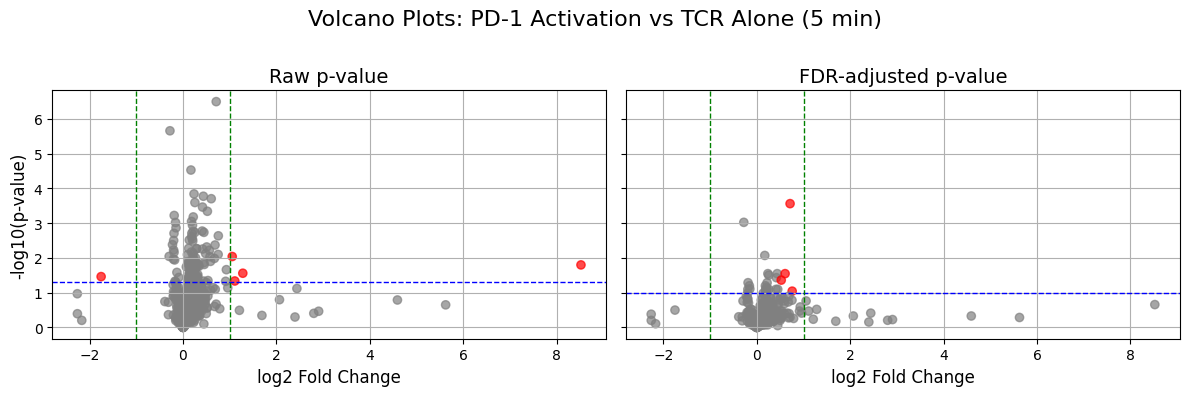
\includegraphics[width=\linewidth]{figures/volcano_plots_5min.png}
              \caption{5 minutes.}
              \label{fig:volcano_plots_5min}
          \end{subfigure}

          \vspace{1em} % Control the spacing between subplots

          % --- 20 minutes ---
          \begin{subfigure}{0.8\textwidth}
              \centering
              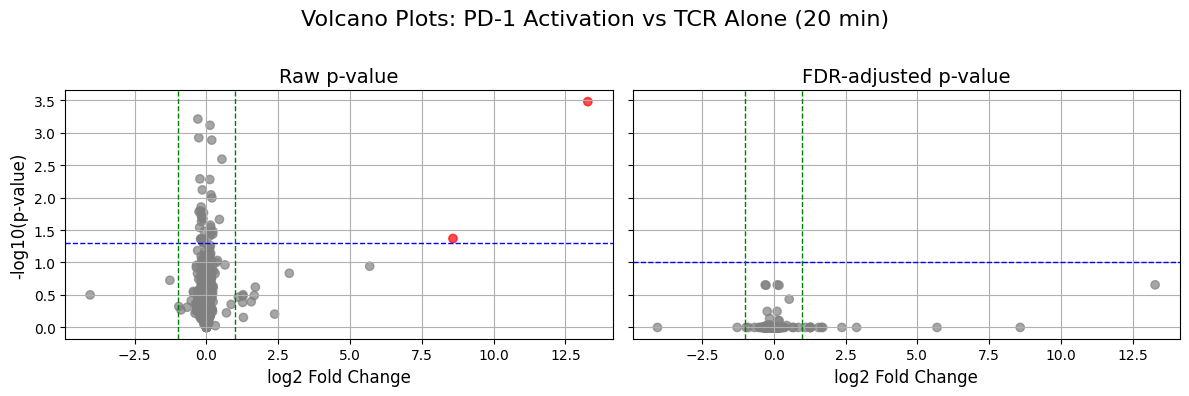
\includegraphics[width=\linewidth]{figures/volcano_plots_20min.png}
              \caption{20 minutes.}
              \label{fig:volcano_plots_20min}
          \end{subfigure}

          \vspace{1em}

          % --- 4 hours ---
          \begin{subfigure}{0.8\textwidth}
              \centering
              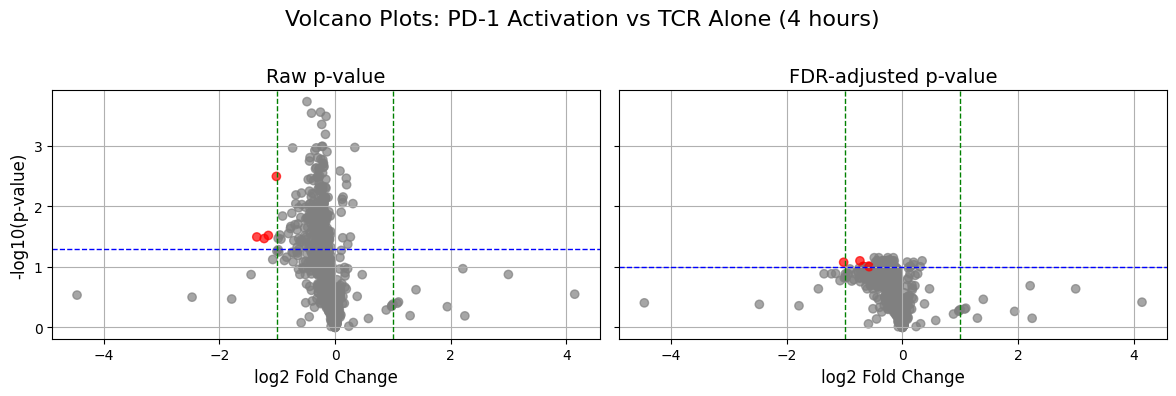
\includegraphics[width=\linewidth]{figures/volcano_plots_4h.png}
              \caption{4 hours.}
              \label{fig:volcano_plots_4h}
          \end{subfigure}

          \caption{Volcano plot analysis results of PD-1 differential expression at multiple time points.}
          \label{fig:volcano_plots}

      \end{figure}

    \subsection{Functional and Pathway Enrichment Analysis}

      \subsubsection{Gene Enrichment Analysis}
      
        Gene set enrichment analysis revealed distinct temporal dynamics following PD-1 activation.

        At 5 minutes, before FDR correction, differentially expressed genes (DEGs) were mainly enriched in GO biological processes related to protein transport, receptor recycling, and metabolic regulation, such as protein retention in the Golgi apparatus, regulation of protein localization, ER-to-Golgi vesicle-mediated transport, and endocytic recycling. Key driver genes included SORL1 and CACTIN. After FDR correction, the number of significant terms decreased, but enrichment remained evident in pathways associated with complement and coagulation cascades, fibrinolysis, regulation of blood coagulation, and immune-related processes (e.g., systemic lupus erythematosus, influenza A infection, cytokine signaling), involving genes such as PLG, HBA2, EWSR1, and H2AC21. These results suggest that PD-1 activation exerts early effects on immune and coagulation-related signaling pathways.

        \begin{table}[H]

          \centering
          \caption{PD-1 differential expression enrichment analysis at 5 minutes (Raw results, top 20).}
          \label{tab:pd1_enrich_raw_5min}

          \resizebox{\textwidth}{!}{%

            \begin{tabular}{@{}llcccc@{}}
              \toprule
              \textbf{Gene set} & \textbf{Term} & \textbf{Overlap} & \textbf{P-value} & \textbf{Adj. P-value} & \textbf{Genes} \\ \midrule
              GO Biological Process 2021 & protein retention in Golgi apparatus (GO:0045053) & 1/5  & 0.001249 & 0.021099 & SORL1 \\
              GO Biological Process 2021 & negative regulation of triglyceride metabolic process & 1/6  & 0.001499 & 0.021099 & SORL1 \\
              GO Biological Process 2021 & regulation of adipose tissue development (GO:1904177) & 1/6  & 0.001499 & 0.021099 & SORL1 \\
              GO Biological Process 2021 & positive regulation of protein localization to membrane (GO:1905744) & 1/8  & 0.001999 & 0.021099 & SORL1 \\
              GO Biological Process 2021 & positive regulation of endocytic recycling (GO:2001134) & 1/8  & 0.001999 & 0.021099 & SORL1 \\
              GO Biological Process 2021 & regulation of protein localization to early endosome (GO:2000643) & 1/8  & 0.001999 & 0.021099 & SORL1 \\
              GO Biological Process 2021 & regulation of aspartic-type endopeptidase activity & 1/9  & 0.002248 & 0.021099 & SORL1 \\
              GO Biological Process 2021 & regulation of ER to Golgi vesicle-mediated transport & 1/9  & 0.002248 & 0.021099 & SORL1 \\
              GO Biological Process 2021 & negative regulation of inclusion body assembly & 1/10 & 0.002498 & 0.021099 & SORL1 \\
              GO Biological Process 2021 & negative regulation of interferon-beta production & 1/10 & 0.002498 & 0.021099 & CACTIN \\
              GO Biological Process 2021 & negative regulation of lipopolysaccharide-mediated signaling & 1/10 & 0.002498 & 0.021099 & CACTIN \\
              GO Biological Process 2021 & receptor recycling (GO:0001881) & 1/10 & 0.002498 & 0.021099 & SORL1 \\
              GO Biological Process 2021 & regulation of tau-protein kinase activity (GO:2000463) & 1/10 & 0.002498 & 0.021099 & SORL1 \\
              GO Biological Process 2021 & positive regulation of cytoplasmic transport (GO:1903829) & 1/11 & 0.002747 & 0.021099 & SORL1 \\
              GO Biological Process 2021 & regulation of endocytic recycling (GO:2001135) & 1/11 & 0.002747 & 0.021099 & SORL1 \\
              GO Biological Process 2021 & regulation of triglyceride catabolic process (GO:0010898) & 1/12 & 0.002997 & 0.021099 & SORL1 \\
              GO Biological Process 2021 & positive regulation of insulin receptor signaling pathway (GO:0046628) & 1/13 & 0.003246 & 0.021099 & SORL1 \\
              GO Biological Process 2021 & positive regulation of protein exit from endoplasmic reticulum (GO:1900100) & 1/13 & 0.003246 & 0.021099 & SORL1 \\
              GO Biological Process 2021 & regulation of protein exit from endoplasmic reticulum (GO:1900101) & 1/13 & 0.003246 & 0.021099 & SORL1 \\ \bottomrule
            \end{tabular}
          }

        \end{table}

        \begin{table}[H]

          \centering
          \caption{PD-1 differential expression enrichment analysis at 5 minutes (FDR-adjusted results, top 20).}
          \label{tab:pd1_enrich_fdr_5min}

          \resizebox{\textwidth}{!}{%

            \begin{tabular}{@{}llcccc@{}}
              \toprule
              \textbf{Gene set} & \textbf{Term} & \textbf{Overlap} & \textbf{P-value} & \textbf{Adj. P-value} & \textbf{Genes} \\ \midrule
              KEGG 2021 Human & African trypanosomiasis & 1/37 & 0.007380 & 0.041638 & HBA2 \\
              KEGG 2021 Human & Malaria & 1/50 & 0.009963 & 0.041638 & HBA2 \\
              KEGG 2021 Human & Complement and coagulation cascades & 1/85 & 0.016893 & 0.041638 & PLG \\
              KEGG 2021 Human & Staphylococcus aureus infection & 1/95 & 0.018866 & 0.041638 & PLG \\
              KEGG 2021 Human & Systemic lupus erythematosus & 1/135 & 0.026730 & 0.041638 & H2AC21 \\
              KEGG 2021 Human & Necroptosis & 1/159 & 0.031425 & 0.041638 & H2AC21 \\
              KEGG 2021 Human & Influenza A & 1/172 & 0.033961 & 0.041638 & PLG \\
              KEGG 2021 Human & Alcoholism & 1/186 & 0.036687 & 0.041638 & H2AC21 \\
              KEGG 2021 Human & Neutrophil extracellular trap formation & 1/189 & 0.037270 & 0.041638 & H2AC21 \\
              KEGG 2021 Human & Transcriptional misregulation in cancer & 1/192 & 0.037853 & 0.041638 & EWSR1 \\
              KEGG 2021 Human & Neuroactive ligand-receptor interaction & 1/341 & 0.066480 & 0.066480 & PLG \\
              GO Biological Process 2021 & negative regulation of fibrinolysis (GO:0051918) & 1/9 & 0.001799 & 0.013914 & PLG \\
              GO Biological Process 2021 & negative regulation of cell-cell adhesion mediated by cadherin & 1/10 & 0.001999 & 0.013914 & PLG \\
              GO Biological Process 2021 & regulation of fibrinolysis (GO:0051917) & 1/13 & 0.002598 & 0.013914 & PLG \\
              GO Biological Process 2021 & fibrinolysis (GO:0042730) & 1/15 & 0.002997 & 0.013914 & PLG \\
              GO Biological Process 2021 & positive regulation of blood coagulation (GO:0030194) & 1/17 & 0.003396 & 0.013914 & PLG \\
              GO Biological Process 2021 & regulation of cell-cell adhesion mediated by cadherin & 1/19 & 0.003795 & 0.013914 & PLG \\
              GO Biological Process 2021 & negative regulation of blood coagulation (GO:0030195) & 1/40 & 0.007977 & 0.018860 & PLG \\
              GO Biological Process 2021 & negative regulation of cell-substrate adhesion (GO:0031589) & 1/40 & 0.007977 & 0.018860 & PLG \\
              GO Biological Process 2021 & negative regulation of cell-cell adhesion (GO:0022408) & 1/41 & 0.008175 & 0.018860 & PLG \\ \bottomrule
            \end{tabular}
          }

        \end{table}

        At 20 minutes, uncorrected results indicated enrichment of processes related to endoplasmic reticulum organization and organelle maintenance, driven primarily by LNPK. However, no significant enrichment was detected after FDR correction, suggesting that PD-1 signaling at this stage may represent a transitional phase, with insufficient molecular perturbations to yield robust enrichment results.

        \begin{table}[H]

          \centering
          \caption{PD-1 differential expression enrichment analysis at 20 minutes (Raw results, top 20).}
          \label{tab:pd1_enrich_raw_20min}

          \resizebox{\textwidth}{!}{%

            \begin{tabular}{@{}llcccc@{}}
              \toprule
              \textbf{Gene set} & \textbf{Term} & \textbf{Overlap} & \textbf{P-value} & \textbf{Adj. P-value} & \textbf{Genes} \\ \midrule
              GO Biological Process 2021 & regulation of endoplasmic reticulum tubular network organization & 1/6   & 0.000600 & 0.003999 & LNPK \\
              GO Biological Process 2021 & cellular component maintenance (GO:0043954) & 1/13  & 0.001300 & 0.003999 & LNPK \\
              GO Biological Process 2021 & endoplasmic reticulum tubular network organization (GO:0071786) & 1/15  & 0.001499 & 0.003999 & LNPK \\
              GO Biological Process 2021 & limb development (GO:0060173) & 1/29  & 0.002898 & 0.005276 & LNPK \\
              GO Biological Process 2021 & positive regulation of organelle organization (GO:0010638) & 1/33  & 0.003297 & 0.005276 & LNPK \\
              GO Biological Process 2021 & endoplasmic reticulum organization (GO:0007029) & 1/73  & 0.007287 & 0.009716 & LNPK \\
              GO Biological Process 2021 & endomembrane system organization (GO:0010256) & 1/199 & 0.019801 & 0.022630 & LNPK \\
              GO Biological Process 2021 & organelle organization (GO:0006996) & 1/420 & 0.041560 & 0.041560 & LNPK \\ \bottomrule
            \end{tabular}
          }

        \end{table}

        At 4 hours, enrichment was dominated by processes associated with protein synthesis and ribosome function. Prior to FDR correction, DEGs were significantly enriched in pathways such as ribosome, cytoplasmic translation, SRP-dependent protein targeting, rRNA metabolism, and mRNA degradation, mainly involving RPLP1, RPL22, and PPIA. After FDR correction, these signals remained robust, with additional enrichment in ribosome biogenesis, rRNA processing, protein translation, and metabolic pathways including the TCA cycle and purine metabolism, involving genes such as EIF6 and NUDT5. These findings indicate that prolonged PD-1 activation strongly suppresses ribosome biogenesis, protein translation, and energy metabolism, consistent with its role in T cell functional inhibition.

        \begin{table}[H]

          \centering
          \caption{PD-1 differential expression enrichment analysis at 4 hours (Raw results, top 20).}
          \label{tab:pd1_enrich_raw_4h}

          \resizebox{\textwidth}{!}{%

            \begin{tabular}{@{}llcccc@{}}
              \toprule
              \textbf{Gene set} & \textbf{Term} & \textbf{Overlap} & \textbf{P-value} & \textbf{Adj. P-value} & \textbf{Genes} \\ \midrule
              KEGG 2021 Human & Ribosome & 2/158 & 0.000368 & 0.001105 & RPLP1; RPL22 \\
              KEGG 2021 Human & Coronavirus disease & 2/232 & 0.000792 & 0.001187 & RPLP1; RPL22 \\
              KEGG 2021 Human & Necroptosis & 1/159 & 0.031425 & 0.031425 & PPIA \\
              GO Biological Process 2021 & SRP-dependent cotranslational protein targeting to membrane & 2/90  & 0.000119 & 0.003128 & RPLP1; RPL22 \\
              GO Biological Process 2021 & cytoplasmic translation (GO:0002181) & 2/93  & 0.000128 & 0.003128 & RPLP1; RPL22 \\
              GO Biological Process 2021 & cotranslational protein targeting to membrane (GO:0006613) & 2/94  & 0.000130 & 0.003128 & RPLP1; RPL22 \\
              GO Biological Process 2021 & protein targeting to ER (GO:0045047) & 2/103 & 0.000157 & 0.003128 & RPLP1; RPL22 \\
              GO Biological Process 2021 & nuclear-transcribed mRNA catabolic process, nonsense-mediated decay (GO:0000184) & 2/113 & 0.000188 & 0.003128 & RPLP1; RPL22 \\
              GO Biological Process 2021 & rRNA metabolic process (GO:0016072) & 2/162 & 0.000387 & 0.004070 & RPLP1; RPL22 \\
              GO Biological Process 2021 & peptide biosynthetic process (GO:0043043) & 2/162 & 0.000387 & 0.004070 & RPLP1; RPL22 \\
              GO Biological Process 2021 & nuclear-transcribed mRNA catabolic process (GO:0000956) & 2/171 & 0.000431 & 0.004070 & RPLP1; RPL22 \\
              GO Biological Process 2021 & rRNA processing (GO:0006364) & 2/173 & 0.000441 & 0.004070 & RPLP1; RPL22 \\
              GO Biological Process 2021 & ribosome biogenesis (GO:0042254) & 2/192 & 0.000543 & 0.004490 & RPLP1; RPL22 \\
              GO Biological Process 2021 & ncRNA processing (GO:0034470) & 2/201 & 0.000595 & 0.004490 & RPLP1; RPL22 \\
              GO Biological Process 2021 & translation (GO:0006412) & 2/214 & 0.000674 & 0.004663 & RPLP1; RPL22 \\
              GO Biological Process 2021 & negative regulation of protein polyubiquitination (GO:0031398) & 1/5   & 0.001000 & 0.006383 & PPIA \\
              GO Biological Process 2021 & negative regulation of stress-activated protein kinase signaling cascade (GO:0032874) & 1/7   & 0.001399 & 0.007808 & PPIA \\
              GO Biological Process 2021 & cellular macromolecule biosynthetic process (GO:0034645) & 2/314 & 0.001444 & 0.007808 & RPLP1; RPL22 \\
              GO Biological Process 2021 & fusion of virus membrane with host plasma membrane (GO:0019064) & 1/8   & 0.001599 & 0.007808 & PPIA \\
              GO Biological Process 2021 & membrane fusion involved in viral entry into host cell (GO:0039654) & 1/8   & 0.001599 & 0.007808 & PPIA \\ \bottomrule
            \end{tabular}
          }

        \end{table}

        \begin{table}[H]

          \centering
          \caption{PD-1 differential expression enrichment analysis at 4 hours (FDR-adjusted results, top 20).}
          \label{tab:pd1_enrich_fdr_4h}

          \resizebox{\textwidth}{!}{%

            \begin{tabular}{@{}llcccc@{}}
              \toprule
              \textbf{Gene set} & \textbf{Term} & \textbf{Overlap} & \textbf{P-value} & \textbf{Adj. P-value} & \textbf{Genes} \\ \midrule
              KEGG 2021 Human & Ribosome & 2/158 & 0.000911 & 0.005466 & RPL18A; RPL22 \\
              KEGG 2021 Human & Coronavirus disease & 2/232 & 0.001949 & 0.005847 & RPL18A; RPL22 \\
              KEGG 2021 Human & Glyoxylate and dicarboxylate metabolism & 1/30  & 0.008967 & 0.013451 & CS \\
              KEGG 2021 Human & Citrate cycle (TCA cycle) & 1/30  & 0.008967 & 0.013451 & CS \\
              KEGG 2021 Human & Ribosome biogenesis in eukaryotes & 1/108 & 0.031969 & 0.038086 & EIF6 \\
              KEGG 2021 Human & Purine metabolism & 1/129 & 0.038086 & 0.038086 & NUDT5 \\
              GO Biological Process 2021 & rRNA processing (GO:0006364) & 3/173 & 0.000012 & 0.000529 & EIF6; RPL18A; RPL22 \\
              GO Biological Process 2021 & ribosome biogenesis (GO:0042254) & 3/192 & 0.000017 & 0.000529 & EIF6; RPL18A; RPL22 \\
              GO Biological Process 2021 & SRP-dependent cotranslational protein targeting to membrane & 2/90  & 0.000297 & 0.004015 & RPL18A; RPL22 \\
              GO Biological Process 2021 & cytoplasmic translation (GO:0002181) & 2/93  & 0.000317 & 0.004015 & RPL18A; RPL22 \\
              GO Biological Process 2021 & cotranslational protein targeting to membrane (GO:0006613) & 2/94  & 0.000324 & 0.004015 & RPL18A; RPL22 \\
              GO Biological Process 2021 & protein targeting to ER (GO:0045047) & 2/103 & 0.000389 & 0.004017 & RPL18A; RPL22 \\
              GO Biological Process 2021 & nuclear-transcribed mRNA catabolic process, nonsense-mediated decay (GO:0000184) & 2/113 & 0.000468 & 0.004142 & RPL18A; RPL22 \\
              GO Biological Process 2021 & rRNA metabolic process (GO:0016072) & 2/162 & 0.000957 & 0.006197 & RPL18A; RPL22 \\
              GO Biological Process 2021 & peptide biosynthetic process (GO:0043043) & 2/162 & 0.000957 & 0.006197 & RPL18A; RPL22 \\
              GO Biological Process 2021 & nuclear-transcribed mRNA catabolic process (GO:0000956) & 2/171 & 0.001066 & 0.006197 & RPL18A; RPL22 \\
              GO Biological Process 2021 & ncRNA processing (GO:0034470) & 2/201 & 0.001468 & 0.006197 & RPL18A; RPL22 \\
              GO Biological Process 2021 & ribose phosphate metabolic process (GO:0019693) & 1/5   & 0.001499 & 0.006197 & NUDT5 \\
              GO Biological Process 2021 & ribosome localization (GO:0033750) & 1/5   & 0.001499 & 0.006197 & EIF6 \\
              GO Biological Process 2021 & mature ribosome assembly (GO:0042256) & 1/5   & 0.001499 & 0.006197 & EIF6 \\ \bottomrule
            \end{tabular}
          }

        \end{table}

        The enrichment results revealed a clear temporal pattern of PD-1–mediated signaling: early perturbation of immune and coagulation pathways at 5 minutes → a transitional state at 20 minutes → robust suppression of translation and metabolism at 4 hours. This time-dependent trajectory aligns with the known immunosuppressive role of PD-1.

      \subsubsection{Cluster Enrichment Analysis}

        After performing Z-value-based cluster analysis and KEGG pathway enrichment analysis on each cluster, I found that different clusters exhibited different functional patterns.

        In Cluster 0, unadjusted results highlighted enrichment in pathways such as Ribosome, Coronavirus disease, and Necroptosis, driven by key genes including RPLP1, RPL22, and PPIA. After FDR correction, Cluster 0 remained strongly enriched in the Ribosome pathway, with additional enrichment in metabolic pathways (e.g., TCA cycle and glyoxylate/dicarboxylate metabolism) as well as the complement and coagulation cascades, involving genes such as RPL18A, RPL22, and CS. These findings suggest that Cluster 0 plays a critical role in translational regulation and metabolic control, with potential links to immune-related processes.

        \begin{table}[H]

          \centering
          \caption{Clustering-based functional enrichment analysis results (without FDR adjustment).}
          \label{tab:cluster_enrich_raw}

          \begin{tabular}{@{}llcc@{}}
            \toprule
            \textbf{Term} & \textbf{Adjusted P-value} & \textbf{Overlap} & \textbf{Genes} \\ \midrule
            \multicolumn{4}{l}{\textbf{Cluster 0 Top 5 KEGG Pathways}} \\ 
            Ribosome & 0.006458 & 2/158 & RPLP1; RPL22 \\
            Coronavirus disease & 0.006857 & 2/232 & RPLP1; RPL22 \\
            Necroptosis & 0.069330 & 1/159 & PPIA \\ \midrule
            \multicolumn{4}{l}{\textbf{Cluster 1 Top 5 KEGG Pathways}} \\
            \multicolumn{4}{c}{No significant pathways detected} \\ \bottomrule
          \end{tabular}

        \end{table}

        In contrast, Cluster 1 showed no significant enrichment before FDR correction. However, after FDR adjustment, this cluster was enriched in several immune- and disease-related pathways, including African trypanosomiasis, Malaria, Systemic lupus erythematosus, Necroptosis, and Alcoholism, primarily driven by HBA2 and H2AC21. This indicates that Cluster 1 is more strongly associated with immune responses and inflammation-related processes.

        \begin{table}[H]

          \centering
          \caption{Clustering-based functional enrichment analysis results (with FDR adjustment).}
          \label{tab:cluster_enrich_fdr}

          \resizebox{\textwidth}{!}{%

            \begin{tabular}{@{}llcc@{}}
              \toprule
              \textbf{Term} & \textbf{Adjusted P-value} & \textbf{Overlap} & \textbf{Genes} \\ \midrule
              \multicolumn{4}{l}{\textbf{Cluster 0 Top 5 KEGG Pathways}} \\ 
              Ribosome & 0.018514 & 2/158 & RPL18A; RPL22 \\
              Coronavirus disease & 0.019705 & 2/232 & RPL18A; RPL22 \\
              Glyoxylate and dicarboxylate metabolism & 0.032833 & 1/30 & CS \\
              Citrate cycle (TCA cycle) & 0.032833 & 1/30 & CS \\
              Complement and coagulation cascades & 0.066628 & 1/85 & PLG \\ \midrule
              \multicolumn{4}{l}{\textbf{Cluster 1 Top 5 KEGG Pathways}} \\
              African trypanosomiasis & 0.014981 & 1/37  & HBA2 \\
              Malaria & 0.014981 & 1/50  & HBA2 \\
              Systemic lupus erythematosus & 0.018811 & 1/135 & H2AC21 \\
              Necroptosis & 0.018811 & 1/159 & H2AC21 \\
              Alcoholism & 0.018811 & 1/186 & H2AC21 \\ \bottomrule
            \end{tabular}
          }

        \end{table}

        The modular analysis highlights a functional division of labor among PD-1-associated proteins: Cluster 0 is mainly involved in translation and metabolic regulation, while Cluster 1 is linked to immune and inflammatory pathways. These results further support the notion that PD-1 signaling orchestrates a dynamic regulation of immune suppression and metabolic inhibition across different time points.

    \subsection{Protein-protein interaction (PPI) network}

      I used the STRING database (v11.5) to construct a protein-protein interaction (PPI) network. For each time point, the significant proteins (both raw and FDR-adjusted) were submitted to STRING with a minimum interaction score of 0.4. Isolated nodes were retained to ensure the complete presentation of the input protein set.

      At the 5-minute time point, the PPI network without FDR adjustment showed several small clusters, including a hemoglobin-related module (HBD, HBG2, HBQ1, HBM, AHSP) and isolated nodes such as CACTIN and HNRNPLL. After FDR correction, the network shifted, highlighting HBA2-centered interactions, including connections with HPX and PLG, suggesting a focus on hemoglobin and coagulation-related pathways.

      \begin{figure}[H]
        \centering
        \begin{subfigure}{0.45\textwidth}
            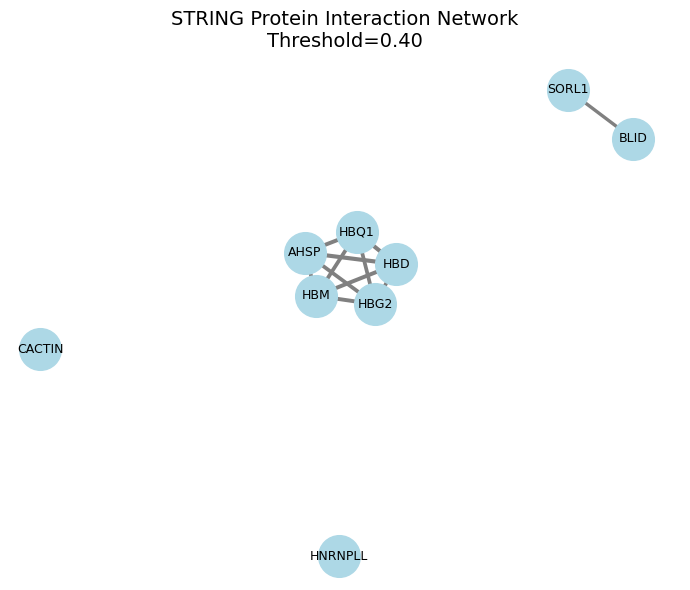
\includegraphics[width=\linewidth]{figures/protein_network_5min.png}
            \caption{Original protein network.}
            \label{fig:protein_network_5min}
        \end{subfigure}
        \hfill
        \begin{subfigure}{0.45\textwidth}
            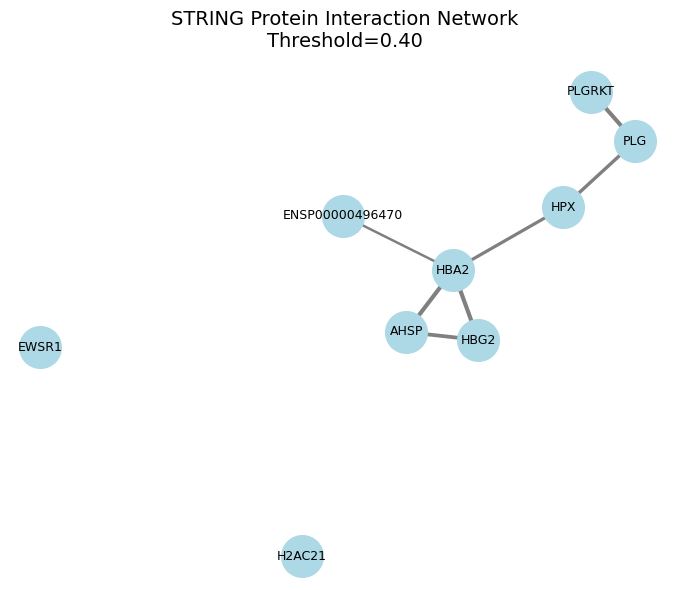
\includegraphics[width=\linewidth]{figures/protein_network_fdr_5min.png}
            \caption{Adjusted protein network.}
            \label{fig:protein_network_fdr_5min}
        \end{subfigure}
        \caption{STRING protein interaction network (5 minutes).}
        \label{fig:protein_network_all_5min}
      \end{figure}

      At the 20-minute time point, the raw results produced a network dominated by LNPK-centered interactions, involving MTX2, HOXD1, and EVX2, while other proteins remained isolated. In contrast, the FDR-adjusted network revealed a more ribosomal-centered module, featuring strong interconnections among RPLP1, RPL22, RPL32, and PPIA, pointing toward translation-related regulation.

      \begin{figure}[H]
        \centering
        \begin{subfigure}{0.45\textwidth}
            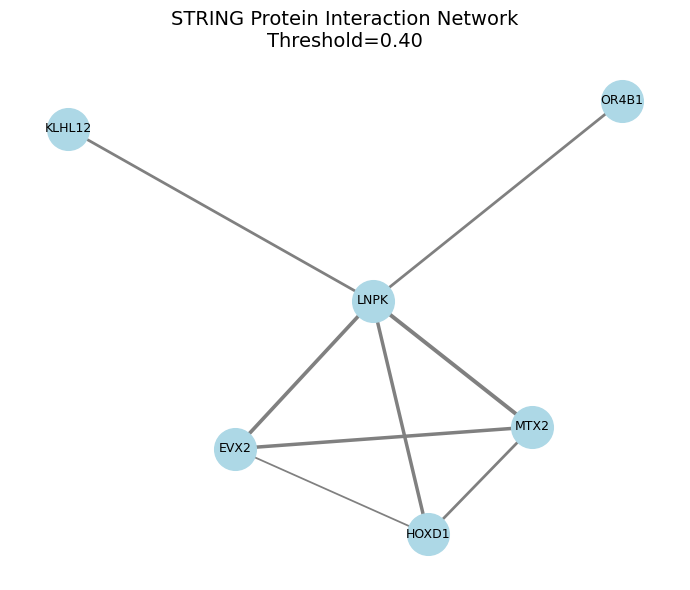
\includegraphics[width=\linewidth]{figures/protein_network_20min.png}
            \caption{Original protein network.}
            \label{fig:protein_network_20min}
        \end{subfigure}
        \hfill
        \begin{subfigure}{0.45\textwidth}
            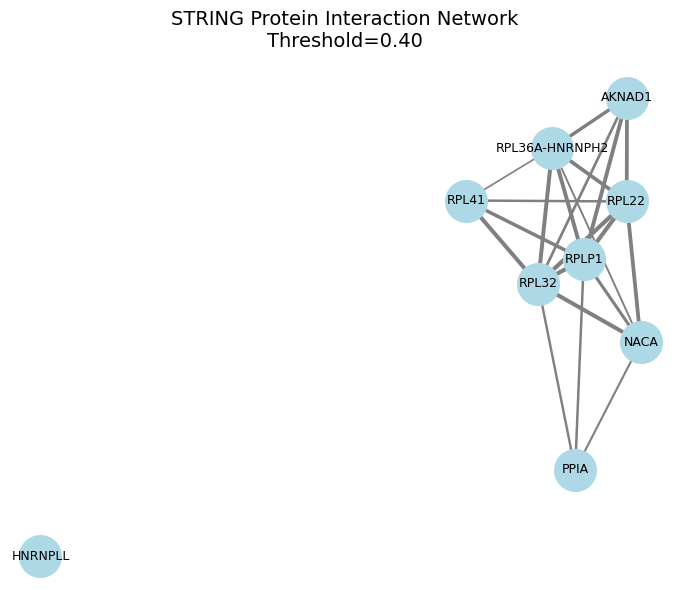
\includegraphics[width=\linewidth]{figures/protein_network_fdr_20min.png}
            \caption{Adjusted protein network.}
            \label{fig:protein_network_fdr_20min}
        \end{subfigure}
        \caption{STRING protein interaction network (20 minutes).}
        \label{fig:protein_network_all_20min}
      \end{figure}

      At the 4-hour time point, both raw and FDR-adjusted analyses showed robust ribosomal protein clusters. In the uncorrected results, RPLP1, RPL22, RPL32, and NACA formed a tightly connected module, whereas after FDR correction, additional ribosomal proteins (RPL18A, RPL36, RPL37, EIF6) appeared, reinforcing ribosome-related functional enrichment. Notably, some isolated nodes such as NUDT5 and CS persisted across conditions, indicating unique functional roles outside the main ribosomal modules.

      \begin{figure}[H]
        \centering
        \begin{subfigure}{0.45\textwidth}
            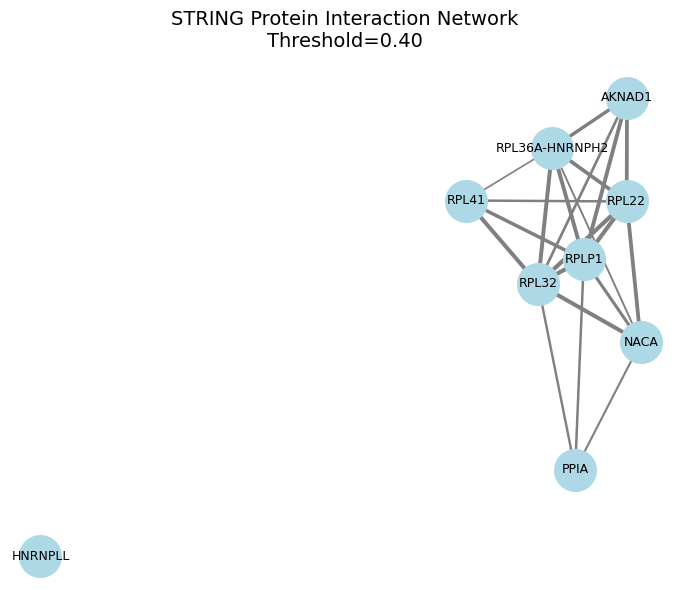
\includegraphics[width=\linewidth]{figures/protein_network_4h.png}
            \caption{Original protein network.}
            \label{fig:protein_network_4h}
        \end{subfigure}
        \hfill
        \begin{subfigure}{0.45\textwidth}
            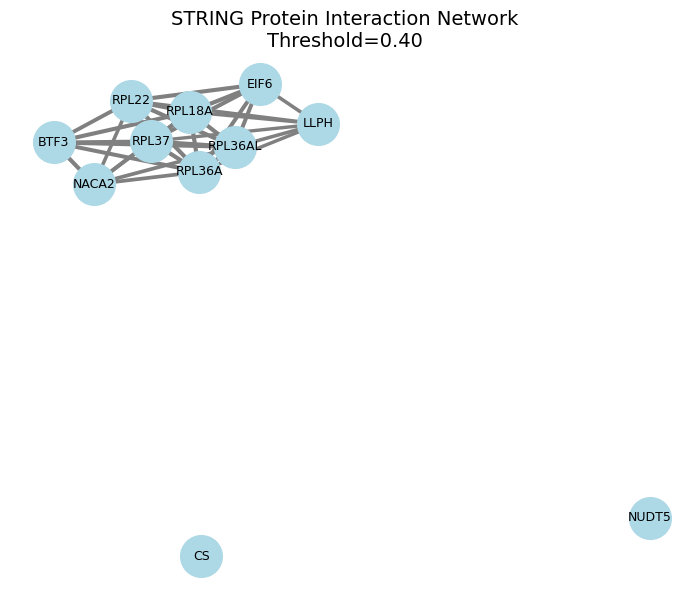
\includegraphics[width=\linewidth]{figures/protein_network_fdr_4h.png}
            \caption{Adjusted protein network.}
            \label{fig:protein_network_fdr_4h}
        \end{subfigure}
        \caption{STRING protein interaction network (4 hours).}
        \label{fig:protein_network_all_4h}
      \end{figure}

      This reflects that PPI analysis revealed changes in the protein interaction network over time following PD-1 activation. Early responses (5 min) were dominated by hemoglobin-associated proteins, while later stages (20 min and 4 h) increasingly converged on ribosomal and translational machinery, suggesting dynamic regulation of cellular processes over time.

    \subsection{Clustering and Visualization}

      To further explore the dynamic expression patterns of the most significant proteins, hierarchical clustering and time-series clustering analyses were performed based on standardized protein expression values (Z-scores). 
      
      \begin{table}[H]
        \centering
        \caption{Top 30 genes Z-score standardization results (with and without FDR correction).}
        \label{tab:zscore_compare}

        \begin{subtable}[t]{0.48\textwidth}
            \centering
            \caption{Without FDR correction.}
            \begin{tabular}{@{}lccc@{}}
              \toprule
              \textbf{Gene} & \textbf{5 min} & \textbf{20 min} & \textbf{4 h} \\ \midrule
              HBD     & 0.1171 & 0.0533 & 0.0810 \\
              RPLP1   & 0.0068 & 0.1338 & 0.0590 \\
              RPL22   & 0.1750 & 0.3426 & 0.2563 \\
              PPIA    & 1.4095 & 1.5725 & 1.1935 \\
              BLTP3A  & 1.0158 & 1.0878 & 1.0873 \\
              H2BC20P & 0.5087 & 0.5219 & 0.5681 \\
              CACTIN  & -0.4728 & -0.6579 & -0.6318 \\
              HNRNPLL & -0.1069 & -0.1986 & -0.0936 \\
              SORL1   & -0.1175 & -2.2597 & 0.0463 \\
              LNPK    & -2.5356 & -0.5957 & -2.5661 \\ \bottomrule
            \end{tabular}
            \label{tab:zscore_raw}
        \end{subtable}
        \hfill
        \begin{subtable}[t]{0.48\textwidth}
            \centering
            \caption{With FDR correction.}
            \begin{tabular}{@{}lccc@{}}
              \toprule
              \textbf{Gene} & \textbf{5 min} & \textbf{20 min} & \textbf{4 h} \\ \midrule
              CS     & -0.4787 & -0.5492 & -0.6580 \\
              PLG    & -0.9230 & -0.9035 & -0.6457 \\
              BTF3   & -1.2416 & -1.1510 & -1.0744 \\
              RPL22  & -0.0271 & 0.2173  & -0.3123 \\
              EIF6   & -0.0654 & -0.2262 & -0.1381 \\
              HBA2   & 1.6264  & 1.7127  & 1.6342 \\
              EWSR1  & -0.1411 & -0.3308 & -0.0366 \\
              RPL18A & -0.4070 & -0.3551 & -0.5148 \\
              H2AC21 & 2.0873  & 2.0243  & 2.1803 \\
              NUDT5  & -0.4299 & -0.4386 & -0.4346 \\ \bottomrule
            \end{tabular}
            \label{tab:zscore_fdr}
        \end{subtable}
    \end{table}
      
      When using the top 30 differential proteins without FDR correction, two distinct temporal trends were observed: one cluster maintained relatively stable expression levels across all time points, while the other exhibited marked fluctuations, particularly at 20 minutes (e.g., SORL1 and LNPK showed strong downregulation at this time point). In contrast, after applying FDR correction, the clustering results revealed a clearer separation between expression profiles. For instance, proteins such as HBA2 and H2AC21 consistently showed strong upregulation, whereas proteins including CS, PLG, and BTF3 remained downregulated throughout the time course. 
      
      \begin{figure}[H]
        \centering
        \begin{subfigure}{0.45\textwidth}
            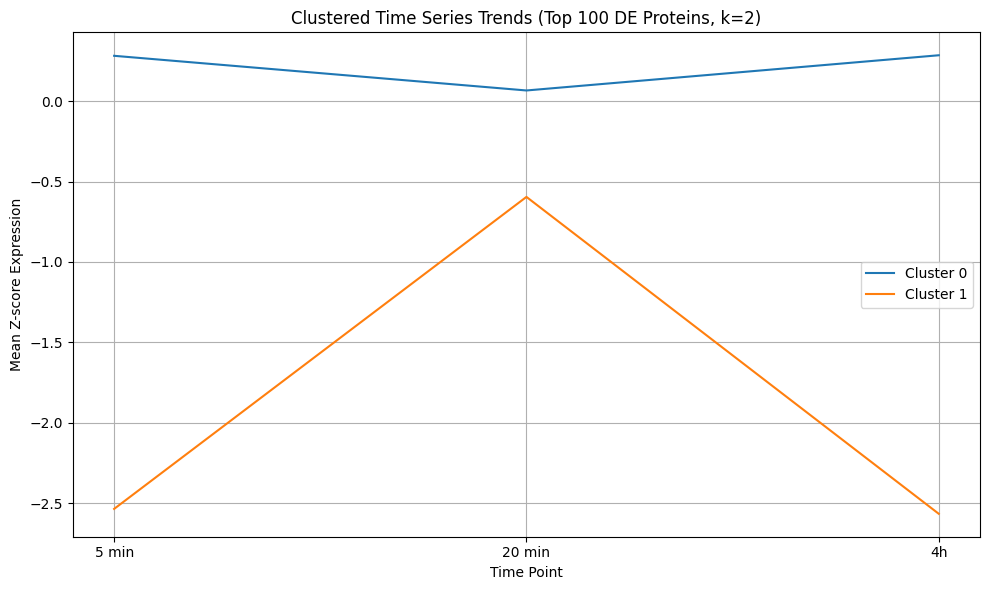
\includegraphics[width=\linewidth]{figures/clustered_time_teries.png}
            \caption{Original clustered time.}
            \label{fig:clustered_time_teries}
        \end{subfigure}
        \hfill
        \begin{subfigure}{0.45\textwidth}
            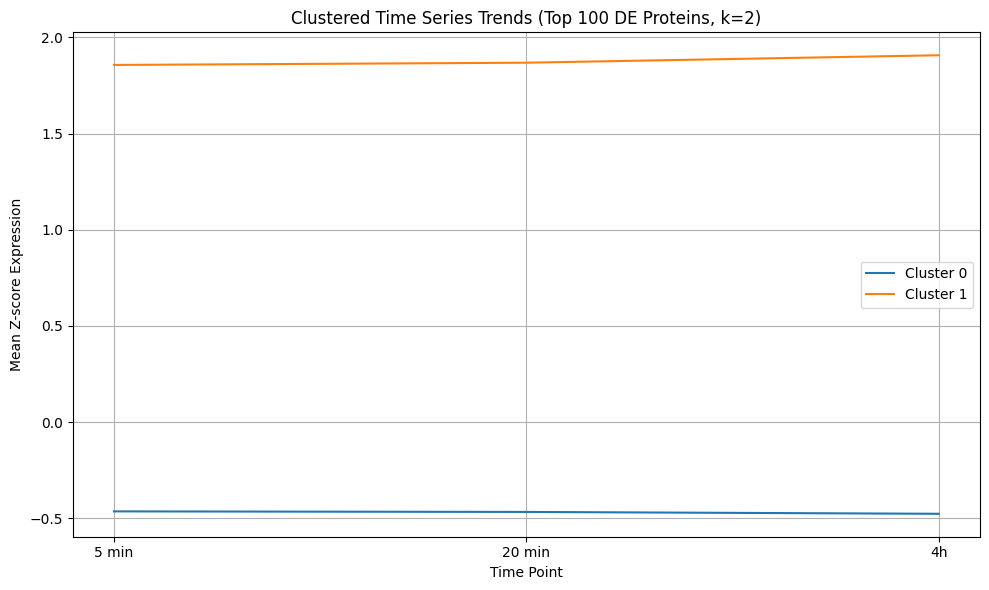
\includegraphics[width=\linewidth]{figures/clustered_time_teries_fdr.png}
            \caption{Adjusted clustered time.}
            \label{fig:clustered_time_teries_fdr}
        \end{subfigure}
        \caption{Clustered time teries analysis.}
        \label{fig:clustered_time_teries_all}
      \end{figure}
      
      The heatmaps further illustrated these clustering differences, with the FDR-adjusted results highlighting more coherent expression modules. 
      
      \begin{figure}[H]
        \centering
        \begin{subfigure}{0.45\textwidth}
            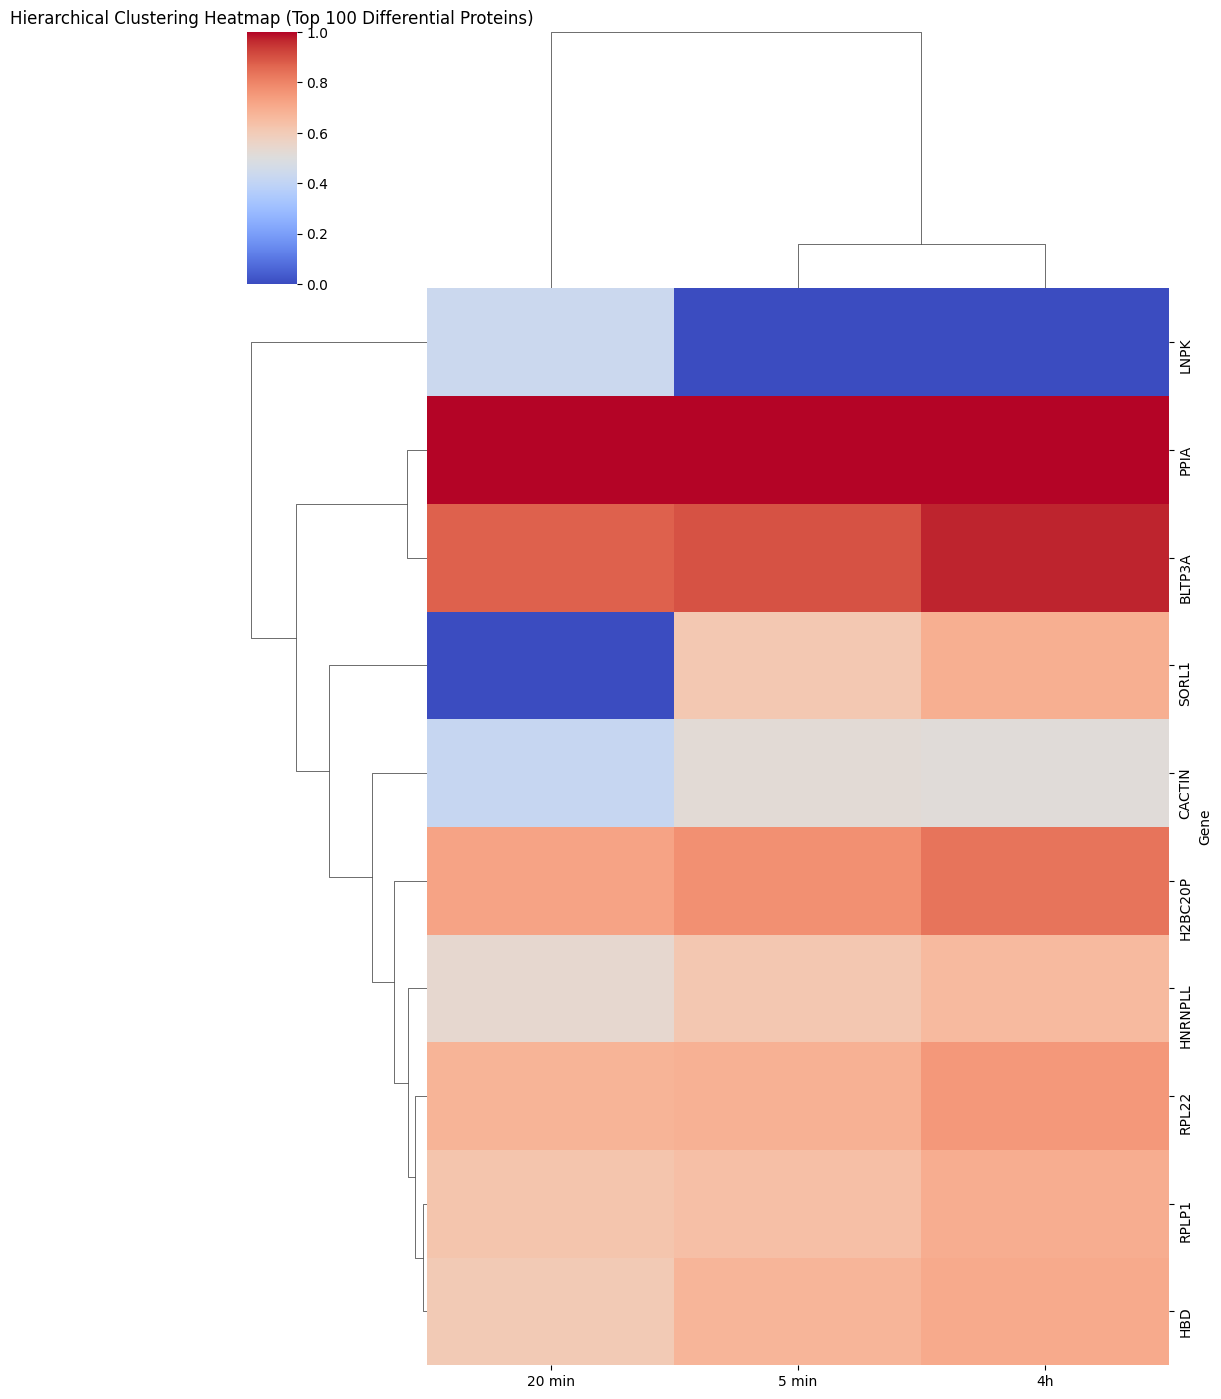
\includegraphics[width=\linewidth]{figures/clustering_heatmap.png}
            \caption{Original clustering heatmap.}
            \label{fig:clustering_heatmap}
        \end{subfigure}
        \hfill
        \begin{subfigure}{0.45\textwidth}
            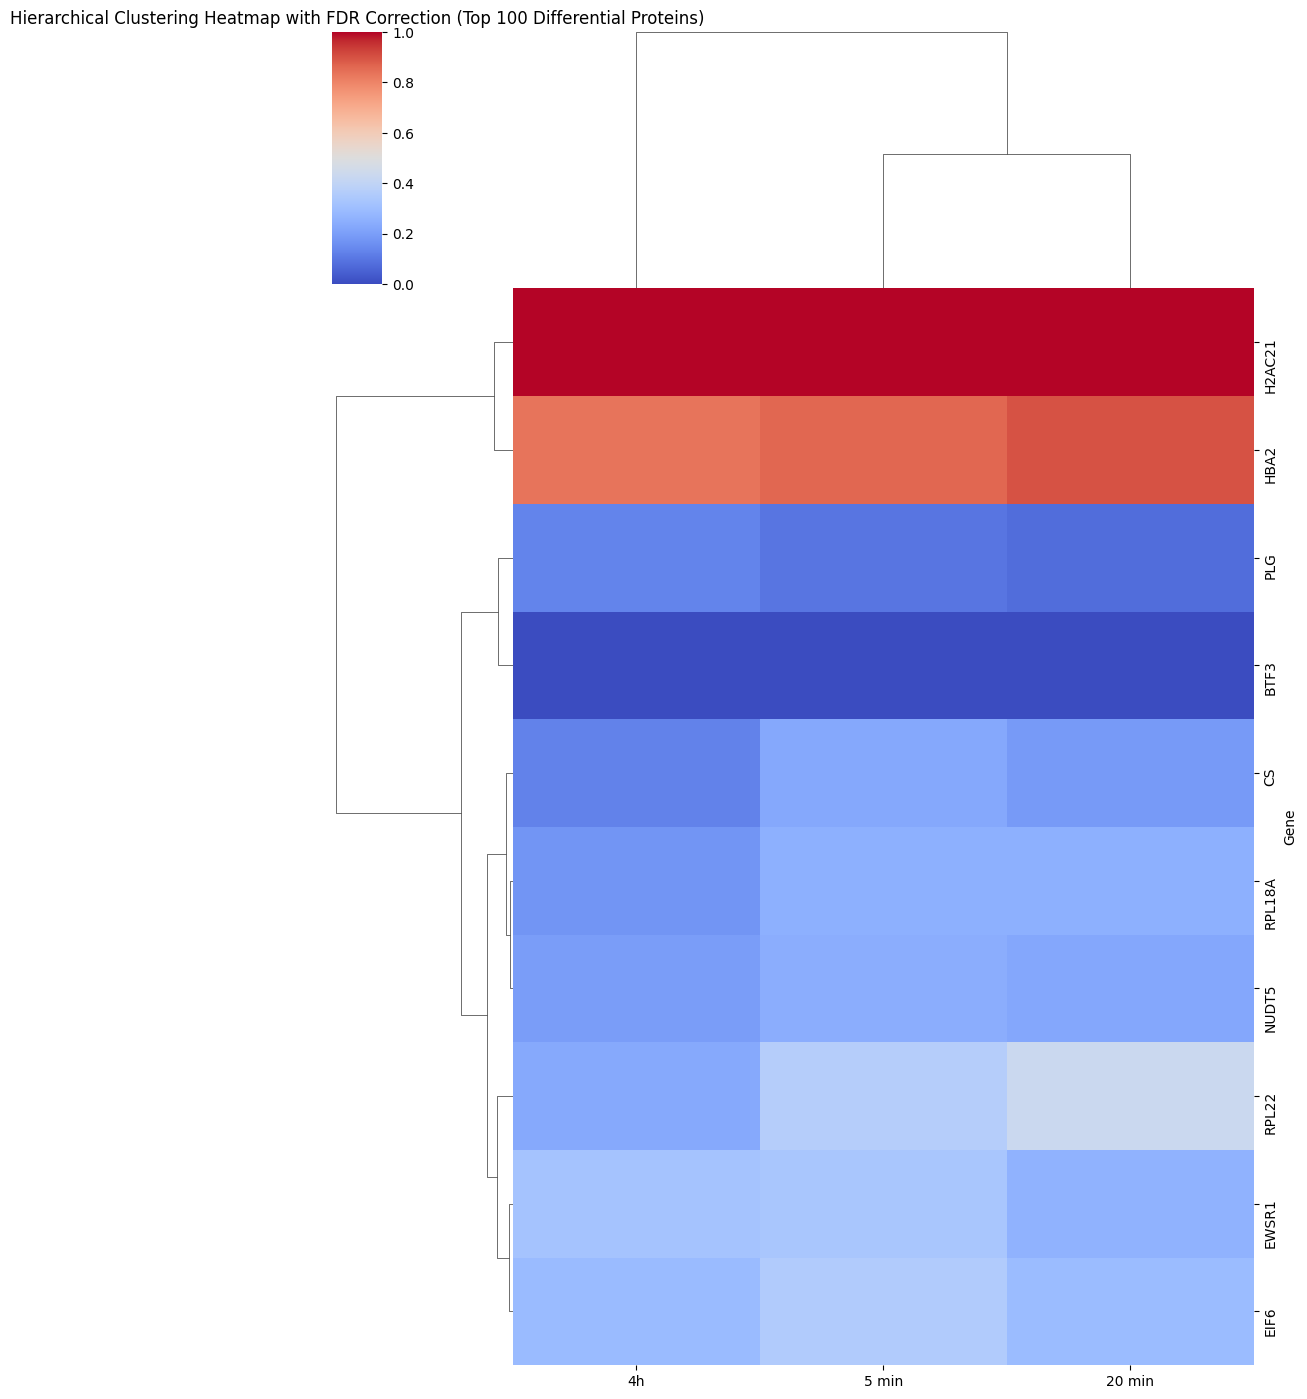
\includegraphics[width=\linewidth]{figures/clustering_heatmap_fdr.png}
            \caption{Adjusted clustering heatmap.}
            \label{fig:clustering_heatmap_fdr}
        \end{subfigure}
        \caption{Clustering heatmap.}
        \label{fig:clustering_heatmap_all}
      \end{figure}
      
      These findings suggest that FDR correction reduces noise and strengthens the identification of biologically relevant protein clusters, thereby providing a more robust interpretation of the temporal proteomic response.

  \section{Conclusions}

    In this project, I systematically profiled the proteomic changes induced by PD-1 activation across multiple time points following TCR stimulation. My analyses revealed that PD-1 signaling exerts time-dependent regulatory effects, with early responses being transient and less stable, while later stages consolidate into more coherent and biologically meaningful proteomic signatures. Differential expression and clustering highlighted both upregulated proteins (e.g., HBA2, H2AC21) and downregulated proteins (e.g., CS, PLG, BTF3), and enrichment analyses linked these clusters to pathways related to ribosomal activity, viral defense, metabolism, and immune regulation. Importantly, applying FDR correction increased the robustness of these findings by reducing false positives and emphasizing biologically relevant modules.

    Taken together, my results provide proteomic-level evidence that PD-1 activation reshapes TCR-driven signaling in a temporally dynamic manner, thereby contributing to a deeper understanding of immune checkpoint inhibitor (ICI) mechanisms. By uncovering key proteins and pathways associated with PD-1-mediated regulation, this work also offers potential insights into the processes underlying resistance development and highlights candidates that may serve as novel therapeutic targets.

  \section*{References}

  {
    \small

    \begin{enumerate}[label={[{\arabic*}]}, leftmargin=*, itemindent=\parindent, align=left, labelsep=0.5em, itemsep=0.25\baselineskip]
      \item Han, Y., Liu, D., \& Li, L. (2020). PD-1/PD-L1 pathway: current researches in cancer. \textit{American Journal of Cancer Research}, \textit{10}(3), 727-742.
      \item Mizuno, R., Sugiura, D., Shimizu, K., Maruhashi, T., Watada, M., Okazaki, I. M., \& Okazaki, T. (2019). PD-1 Primarily Targets TCR Signal in the Inhibition of Functional T Cell Activation. \textit{Frontiers in immunology}, \textit{10}, 630. \url{https://doi.org/10.3389/fimmu.2019.00630}.
      \item Chen, H. Z., Kim, N. H., Nishizaki, D., Nesline, M. K., Conroy, J. M., DePietro, P., ... \& Kurzrock, R. (2025). PD-1 transcriptomic landscape across cancers and implications for immune checkpoint blockade outcome. \textit{NPJ Genomic Medicine}, \textit{10}(1), 21. \url{https://doi.org/10.1038/s41525-025-00465-9}.
      \item Hasselmo, M. E., Schnell, E., \& Barkai, E. (1995). Dynamics of learning and recall at excitatory recurrent synapses and cholinergic modulation in rat hippocampal region CA3. \textit{Journal of Neuroscience}, \textit{15}(7), 5249-5262.
    \end{enumerate}
  }

\end{document}